\RequirePackage{plautopatch}
\documentclass[dvipdfmx,a4paper]{jsarticle}
\usepackage{graphicx}

\usepackage{amsmath}
\usepackage{amssymb}
\usepackage{float}
\usepackage{tikz}
\usepackage{pgfplots}
\pgfplotsset{compat=1.18}
\usepackage{geometry}
\geometry{a4paper, margin=2.5cm} % 余白を設定

\title{船体運動力学課題3}
\author{08C23031 \\ 古賀 光一朗}
\date{2025年7月6日}

\begin{document}

\maketitle

波浪中の船体運動を定義する座標系を模式的に下図に示す。
船体はある一定の速度 $u_c$ で $X_1$ 軸の正方向に進んでいるとする。
船は左右対称・前後非対称の単胴船とする。

\begin{figure}[H]
    \centering
    % 画像ファイル名を適切に設定してください
    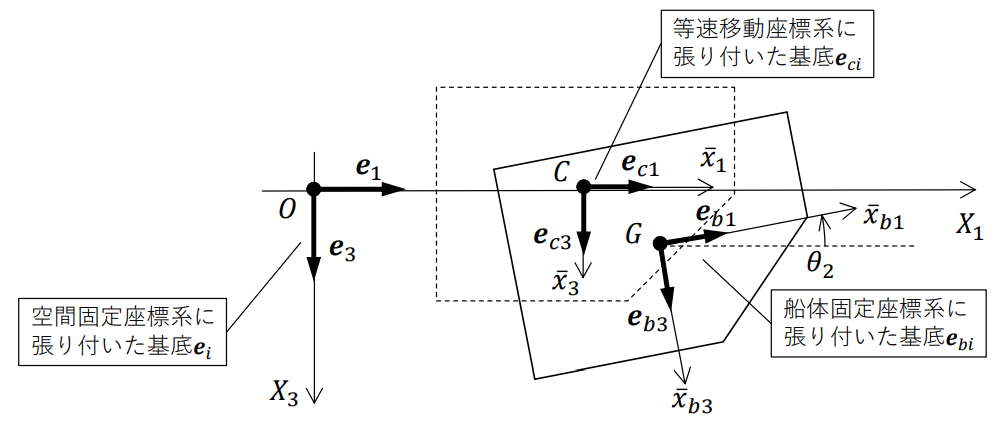
\includegraphics[width=0.9\linewidth]{summer/ship-dynamics/day3/day3_01.png} 
    \caption{船体運動に関する座標系}
    \label{fig:coordinates}
\end{figure}

規則波中では、船体はC点まわりに速度で運動し、それは空間固定座標から見ると $\boldsymbol{u}_G$ の速度である。
このとき、運動方程式は慣性座標系で次の通りに示される。

$$ M\dot{\boldsymbol{u}}_G = -A\dot{\boldsymbol{u}}_G - B\boldsymbol{u}_G - C\boldsymbol{x}_G - A'\dot{\boldsymbol{\omega}} - B'\boldsymbol{\omega} - C'\boldsymbol{\theta} + \boldsymbol{f}_e(t) $$
$$ I\dot{\boldsymbol{\omega}} = -\overline{A}\dot{\boldsymbol{u}}_G - \overline{B}\boldsymbol{u}_G - \overline{C}\boldsymbol{x}_G - \overline{A}'\dot{\boldsymbol{\omega}} - \overline{B}'\boldsymbol{\omega} - \overline{C}'\boldsymbol{\theta} + \boldsymbol{q}_e(t) $$

ここで、$\boldsymbol{u}_G, \boldsymbol{x}_G$ はそれぞれ重心の速度ベクトル、変位ベクトルであり、$\boldsymbol{\omega}, \boldsymbol{\theta}$ は角速度ベクトル、角度ベクトルを表す。
$M, I$ はそれぞれ慣性マトリクス、回転慣性マトリクスである。
$\boldsymbol{f}_e, \boldsymbol{q}_e$ はそれぞれ波強制力ベクトル、波強制力モーメントベクトルである。

\subsection*{(1) $\boldsymbol{u}, \boldsymbol{u}_C, \boldsymbol{u}_G$ の関係を示しなさい。}
空間固定座標系から見た船体重心 $G$ の速度 $\boldsymbol{u}_G$ は、等速で並進する移動座標系の原点 $C$ の速度 $\boldsymbol{u}_C$ と、移動座標系から見た重心 $G$ の相対速度 $\boldsymbol{u}$ のベクトル和として表される。
したがって、これらの関係は以下の式で示される。
$$
\boldsymbol{u}_G = \boldsymbol{u}_C + \boldsymbol{u}
$$

\subsection*{(2) $A, B, C$ は一般に何と呼ばれるか。}
\begin{itemize}
    \item \textbf{$A$ : 付加質量} 
    \item \textbf{$B$ : 減衰力係数}
    \item \textbf{$C$ : 復原力係数} 
\end{itemize}

\subsection*{(3) Radiation force (ラディエイション力) と波強制力の違いについて説明しなさい。}
ラディエイション力は\textbf{造波減衰力}と\textbf{負荷慣性力}から成り、船が運動することにより作用するが、
波強制力は船の運動に関係なく作用する

\subsection*{(4) 平水中(入射波が無い状態)で動揺している船体は、時間がたつと動揺がおさまる。 動揺がおさまる原理を説明しなさい。}
平水中(入射波がない状態)で動揺する船体が時間とともにおさまるのは、船体の運動エネルギーが、主に\textbf{造波減衰}によって失われるためである。

船体が前後揺, 上下揺, 縦揺などで船体表面が水を押し、造波抵抗を受ける。この波はエネルギーを持っており、波が遠くへ去っていくことは、船体の運動エネルギーが波のエネルギーとして周囲の水中へ放出されていくことを意味する。
エネルギー保存則により、船体系からエネルギーが失われ続けるため、船体の運動エネルギーは徐々に減少し、振幅が小さくなっていく。最終的には運動エネルギーがゼロになり、動揺は完全におさまる。
\vfill
\end{document}